\chapter{Project Design}

In this section we demonstrate, using Unified Modeling Language(UML) notation, the conceptual model using  ''use cases'' diagrams(taking the functional requirements into account), The architecture of the System and database design using Class Diagrams and  Sequence Diagrams between key processes.(list and expand on the functional requirements there where necessary)
\section{Functional Requirements}
\begin{itemize}
\item registration of admin and clients
\item enable logging in and logging out 
\item allow users(both admin and clients) to view dashboard
\item allow clients to add/revoke a rental offer
\item allow clients to add/remove details of rental offer
\item allow clients to add/remove photos of offer
\item allow admins to browse clients and client details
\item allow admins to edit content of user
\item allow users to browse offers based on criteria 
\item allow users to make bookings and confirm bookings
\item allow users to rate room based on criteria offered
\item allow landlords to anonymously rate client
\item allow users to edit personal details 
\item create password resetting facilities
\item allow basic content management
\item create easy to use application programming interface(API)
\end{itemize}
\clearpage
\section{Users, roles and use case}
\begin{figure}[h!]
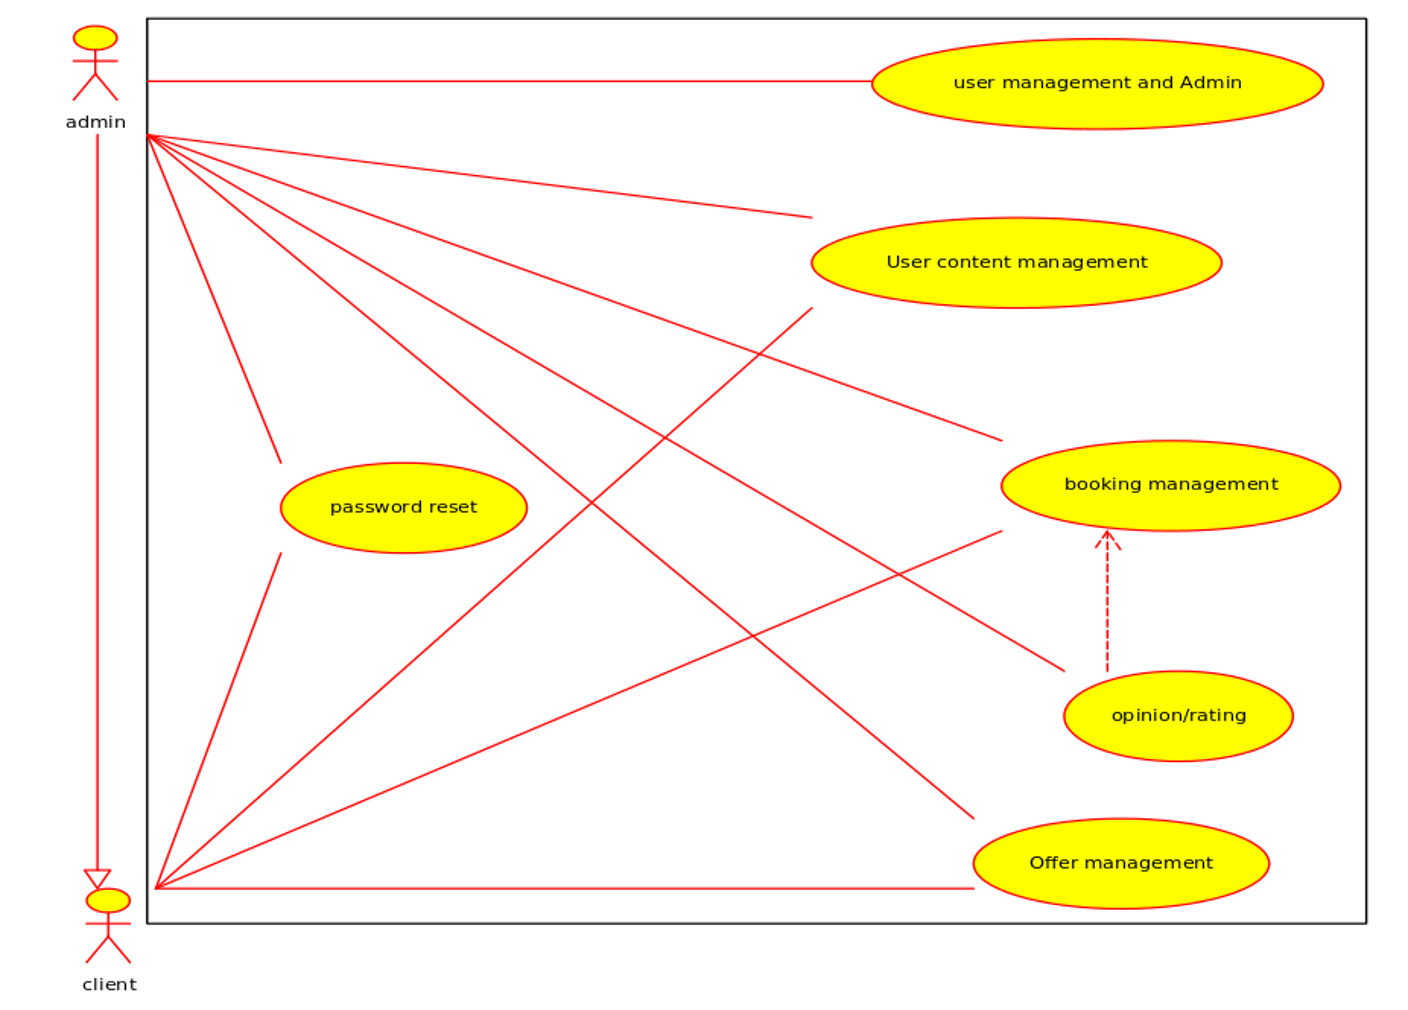
\includegraphics[scale=0.3]{img/updated_use_case.jpg}
\caption{details}
\end{figure}
The project consists of two groups of users whom access and modify a database of information via a user interface. These users are:
\begin{itemize}
\item Administrator 
\item Client(landlord and regular)
\end{itemize}
\newpage
\section{Architecture}
\section{Database Design}
\section{Sequence Diagrams}
\section{Protocols}